% DOCUMENTO PRINCIPAL

% Este es el fichero principal de este repositorio. No se recomienda editarlo.
% Modifica las plantillas incluidas en los directorios:
% - secciones
% - tablas
% - algoritmos

\documentclass[final,a4paper,11pt,twoside]{class_diss}

\usepackage[full]{textcomp}
\usepackage{graphicx}
\usepackage{amsmath}
\usepackage{amsxtra}
\usepackage{amssymb}
\usepackage{amsthm}
\usepackage{latexsym}
\usepackage{setspace}
\usepackage[margin=3cm]{geometry}
\usepackage[titles]{tocloft}
\usepackage{latexsym}
\usepackage{fancyhdr}
\usepackage{emptypage}
\usepackage[svgnames,dvipsnames,usenames,table,xcdraw]{xcolor}
\usepackage{tikz}
\usepackage[toc,acronym,nonumberlist,xindy={language=spanish-traditional},sanitize=none]{glossaries}
\usepackage[scaled]{helvet}
\usepackage[utf8]{inputenc}
\usepackage[T1]{fontenc}
\usepackage[spanish,es-tabla]{babel}
\usepackage[explicit]{titlesec}
\usepackage{newtxtext}
\usepackage{newtxmath}
\usepackage{stmaryrd}
\usepackage{bbold}
\usepackage[ruled,vlined]{algorithm2e}
\usepackage{algorithmic}
\usepackage{float}
\usepackage{url}
\usepackage{xspace}
\usepackage{booktabs}
\usepackage{multirow}
\usepackage{enumitem}
\usepackage{rotating}
\usepackage{pdflscape}
\usepackage{pdfpages}
\usepackage{listings}
\usepackage{placeins}
\usepackage{flafter}

\theoremstyle{definition}
\newtheorem{definition}{Teorema}[section]
\theoremstyle{remark}
\newtheorem*{remark}{Remark}
\DeclareMathOperator*{\argmax}{arg\,max}
\DeclareMathOperator*{\argmin}{arg\,min}
\definecolor{VIU}{RGB}{240, 90, 15}
\definecolor{DESTACADO}{RGB}{130, 34, 145}
\definecolor{CITA}{RGB}{0, 123, 194}

\renewcommand{\algorithmcfname}{Algoritmo}
\renewcommand{\acronymname}{Lista de Acr\'onimos}
\addto\captionsspanish{
    \renewcommand*{\acronymname}{Lista de Acr\'onimos}
}
\newcommand{\inhib}{\relbar\mapsfromchar}
\newcommand{\destacado}[1]{\color{DESTACADO}\textbf{#1}\color{black}\xspace}

\usetikzlibrary{shapes}
\newcommand*\circled[1]{\tikz[baseline=(char.base)]{
    \node[shape=diamond,fill=black!90,inner sep=1pt,minimum size=1cm] (char) {\textcolor{white}{\small\textbf{#1}}};}
}

\pagestyle{fancy}
\fancyhf{}
\fancyhead[LO]{}
\fancyhead[RE]{}
\fancyfoot[C]{}
\renewcommand{\headrulewidth}{0pt}

\fancypagestyle{plain}{
  \fancyhf{}
  \fancyfoot[C]{\circled{\thepage}}
  \renewcommand{\headrulewidth}{0pt}
}

\colorlet{chapnumcolor}{VIU}

\newcommand*{\chapnumfont}{%
  \usefont{T1}{jkp}{b}{n}%
  \fontsize{70}{90}%
  \selectfont%
}

\newcommand*{\chaptitlefont}{%
  \usefont{T1}{qhv}{b}{n}%
  \fontsize{22}{26}%
  \selectfont%
}

\titleformat{name=\chapter}
{\normalfont\huge\bfseries}
{\rlap{\parbox{\textwidth}{\filleft\chapnumfont\color{chapnumcolor}\thechapter}}}
{0pt}
{\rlap{\parbox{0.7\textwidth}{\filright\chaptitlefont #1}}}

\makeglossaries
% GLOSARIO

% Si quieres incluir un glosario y una lista de abreviaturas en tu Trabajo Fin de Máster,
% sigue las instrucciones indicadas en la siguiente URL:
% https://www.overleaf.com/learn/latex/glossaries

\newacronym{gan}{GAN}{Red Generativa Antagónica o \textit{Generative Adversarial Network}}


\bibliographystyle{apa}

\usepackage[authoryear,sort&compress]{natbib}
\usepackage{hypernat}
\setcitestyle{authoryear}

\usepackage[pdftex,plainpages=false,pdfpagelabels]{hyperref}

\hypersetup{
    linktocpage=true,
    colorlinks=true,
    bookmarks=true,
    citecolor=CITA,
    urlcolor=CITA,
    linkcolor=CITA,
    citebordercolor={1 0 0},
    urlbordercolor={1 0 0},
    linkbordercolor={.7 .8 .8},
    breaklinks=true,
    pdfpagelabels=true,
    }

\setcounter{secnumdepth}{3}
\onehalfspacing
\renewcommand\familydefault{\sfdefault}

\begin{document}

%%%% Incluye la portada oficial%%%%
%% Archivo portada.docx
\cleardoublepage

% Escribe aquí tu frase favorita
\null\vspace{\stretch{2}}
{
\hfill \begin{minipage}{8cm}
\textsl{
\begin{flushright}
    Escribe aquí \\ tu frase favorita.
\end{flushright}
}

% E indica aquí su autor
\begin{flushright}
E indica aquí su autor
\end{flushright}

\end{minipage}
}
\vspace{\stretch{1}}


\pagenumbering{gobble}
% AGRADECIMIENTOS

\cleardoublepage

\normalfont{\huge{\bfseries{Agradecimientos}}}
\vspace{15ex}

% Escribe tus agradecimientos a continuación.
% Se recomienda separar cada párrafo con un \medskip.

A mi familia. 
A mis padres y a mis hermanos.
\medskip
\cleardoublepage

\newpage
\pagenumbering{roman}
\setcounter{page}{1}

\pagestyle{fancy}
\fancyhf{}
\fancyhead[LO]{\leftmark}
\fancyhead[RE]{\rightmark}
\fancyfoot[C]{\circled{\thepage}}
\renewcommand{\headrulewidth}{0.4pt}

\pdfbookmark[0]{\contentsname}{contents}

\renewcommand{\cftchapleader}{\cftdotfill{\cftdotsep}}
\renewcommand{\cftchapfont}{\mdseries}
\renewcommand{\cftchappagefont}{\mdseries}

\tableofcontents
\listoffigures
\listoftables

\renewcommand{\listalgorithmcfname}{Índice de algoritmos}
\listofalgorithms
\addcontentsline{toc}{chapter}{Índice de algoritmos}

\newpage
\pagenumbering{arabic}
\setcounter{page}{1}

\cleardoublepage

\chapter*{Resumen}
\label{resumen}
\addcontentsline{toc}{chapter}{Resumen}

El siguiente trabajo presenta una alternativa mediante el uso de técnicas de aprendizaje por refuerzo al algoritmo de seguimiento de una persona en tiempo real por parte de un dron. A diferencia de estudios ya realizados anteriormente y los cuales iremos detallando a lo largo del siguiente documento, no utilizaremos simuladores para la obtención de los datos, sino que utilizaremos la propia cámara del dispositivo para obtener estos, de manera que el entorno final sea lo más parecido al entorno de entrenamiento.


Construiremos en primer lugar una base teórica, en la que explicaremos brevemente los conceptos que involucra el siguiente trabajo y que da pie a entender las diferentes decisiones tomadas durante su ejecución.


Luego realizaremos un análisis de nuestros objetivos, tomaremos la definición de nuestro problema, y lo estructuraremos para adaptarlo al modelo de problema de aprendizaje por refuerzo. Además iremos comentando los problemas que cada uno de estos pasos conlleva y su evolución y distintas variantes a lo largo de los diferentes experimentos, incluyendo decisiones en el entrenamiento de nuestros agentes, así como la redefinición y adaptación mediante análisis de resultados, pero también mediante prueba y error de cada una de las piezas.


Finalmente haremos un análisis de los algoritmos utilizados y trataremos los diferentes problemas que estos fueron ocasionando durante el transcurso del entrenamiento. 


% INTRODUCCIÓN

\cleardoublepage

\chapter{Introducción}
\label{introduccion}

El objetivo es poder realizar el seguimiento a tiempo real de una persona a través de la cámara del dispositivo utilizando para ello visión por computador y técnicas de aprendizaje por refuerzo para controlar las acciones a tomar en cada momento. Lo que se conoce como active tracking. 
\medskip

Los recientes algoritmos y estudios alrededor del \textit{active tracking}, entre ellos \citet{activetracking} o \citet{zhou2021space}, se centran fundamentalmente en el reconocimiento del objeto y en la posición de éste con respecto a las coordenadas X e Y en relación al centro de la imagen a través de la cámara incorporada para guiar las acciones del dispositivo. Es lo que se conoce como \textit{passive tracking}. Este tipo de algoritmos han ganado más atención debido a la simplicidad del problema y los avances en reconocimiento de objetos.
\medskip

Otros intentos de realizar \textit{object tracking} con aprendizaje supervisado se realizan utilizando modelos en simuladores tanto del dron como de las personas. Sin embargo, la idea del presente trabajo es la aplicación de diferentes técnicas de inteligencia artificial para lograr un agente que sea capaz de realizar el seguimiento utilizando simplemente imágenes que provengan del propio dispositivo en el cual se desplegará el agente.
\medskip

\begin{figure}[ht!]
\centering
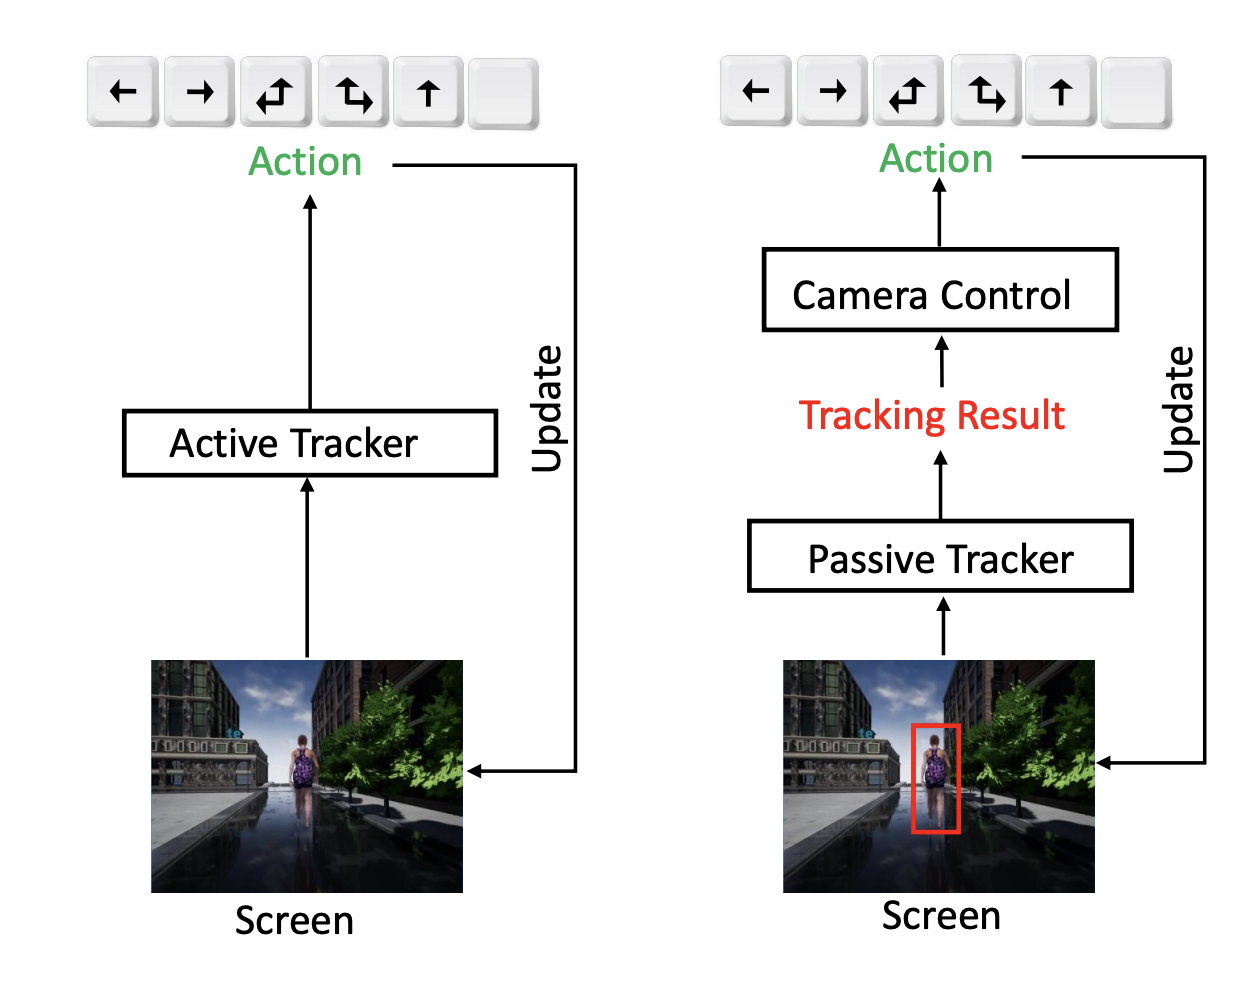
\includegraphics[scale=0.4]{figuras/active_tracking_vs_passive_tracking.png}
\caption[A la izquierda, el pipeline utilizado durante active tracking. A la derecha, el pipeline utilizado en passive tracking.]{A la izquierda, el pipeline utilizado durante active tracking. A la derecha, el pipeline utilizado en passive tracking. Imagen tomada de \citet{luo2019end}.}
\label{fig-active-tracking}
\end{figure}
\medskip

Para ello, no solo utilizaremos técnicas de aprendizaje por refuerzo, sino también técnicas de aprendizaje supervisado para la obtención de nuestro conjunto inicial.
\medskip

El desarrollo del proyecto se llevará a cabo utilizando lenguaje Python y la librería \href{https://pytorch.org/}{PyTorch} para el desarrollo de los modelos. El código completo estará disponible para su visualización en un repositorio de \href{https://github.com/lucaswerner90/msc-degree-ai}{GitHub}, a excepción de los pesos de los diferentes agentes que se vayan guardando durante el entrenamiento debido al tamaño individual de cada uno de estos archivos.


\section{Acotación del problema}
\label{acotacion-del-problema}

Debido a que nos movemos en un entorno real, en el cual las posibilidades son muy amplias, no solo debido a la aleatoriedad del mismo sino también al número de acciones que podemos tomar, debemos definir ciertas restricciones.
\medskip

En primer lugar, nos centraremos en obtener una solución que sea viable en entornos en los cuales las condiciones externas no sean un impedimento para el buen funcionamiento de nuestro algoritmo. Esto quiere decir que durante el desarrollo y testeo de los algoritmos obviamos factores tales como el viento, las condiciones de humedad o el grado de iluminación en un momento dado, que pudiesen afectar al rendimiento del dispositivo.
\medskip

Por otro lado, debido a que el espacio de acciones disponibles es muy alto, en una primera fase dispondremos de tan solo 3: 

\begin{itemize}
  \item Girar a la derecha.
  \item Girar a la izquierda.
  \item Mantenerse en el mismo lugar.
\end{itemize}
\medskip

Tanto el giro a la derecha como el giro a la izquierda se realizará en el dispositivo de manera controlada, esto quiere decir que nos moveremos siempre utilizando el mismo ángulo de giro. Si quisiéramos añadir además un ángulo de giro variable junto con la acción a tomar podríamos hacerlo como parte de la salida de nuestro algoritmo, aunque involucraría un entrenamiento más prolongado en el tiempo y se escaparía a las restricciones de tiempo de este proyecto.
\medskip

De tal forma que nuestra solución será valorada positiva o negativamente con respecto al eje X exclusivamente. Esto quiere decir que consideraremos que el algoritmo funciona de forma correcta si es capaz de moverse de tal manera que la persona se encuentre siempre centrada en el eje horizontal y no en el eje vertical.
\medskip

En cuanto a la detección de la persona, tenemos en cuenta que nuestro dispositivo solo realizará el seguimiento de una sola persona, debido a la complejidad que esto supondría en cuanto al funcionamiento de nuestro algoritmo. Obviamos un escenario real y plausible que es el de encontrarnos en una misma imagen con múltiples personas, en cuyo caso deberíamos también de desarrollar un mecanismo de selección de la persona a la cual quisiéramos seguir.
\medskip

Por lo tanto, quedándonos con una parte simplificada del problema, podemos centrarnos en conseguir un algoritmo que pueda considerarse como el mínimo viable para conseguir nuestro objetivo.
\medskip

\section{Dispositivo utilizado}
\label{dispositivo-utilizado}

Para el desarrollo del proyecto se utilizará el dispositivo \href{https://store.dji.com/de/shop/tello-series}{DJI Tello}, ya que nos proporciona una interfaz de programación compatible con nuestras necesidades: control del dispositivo y transmisión de datos a través de una API en lenguaje Python.
\medskip


\begin{figure}[ht!]
  \centering
  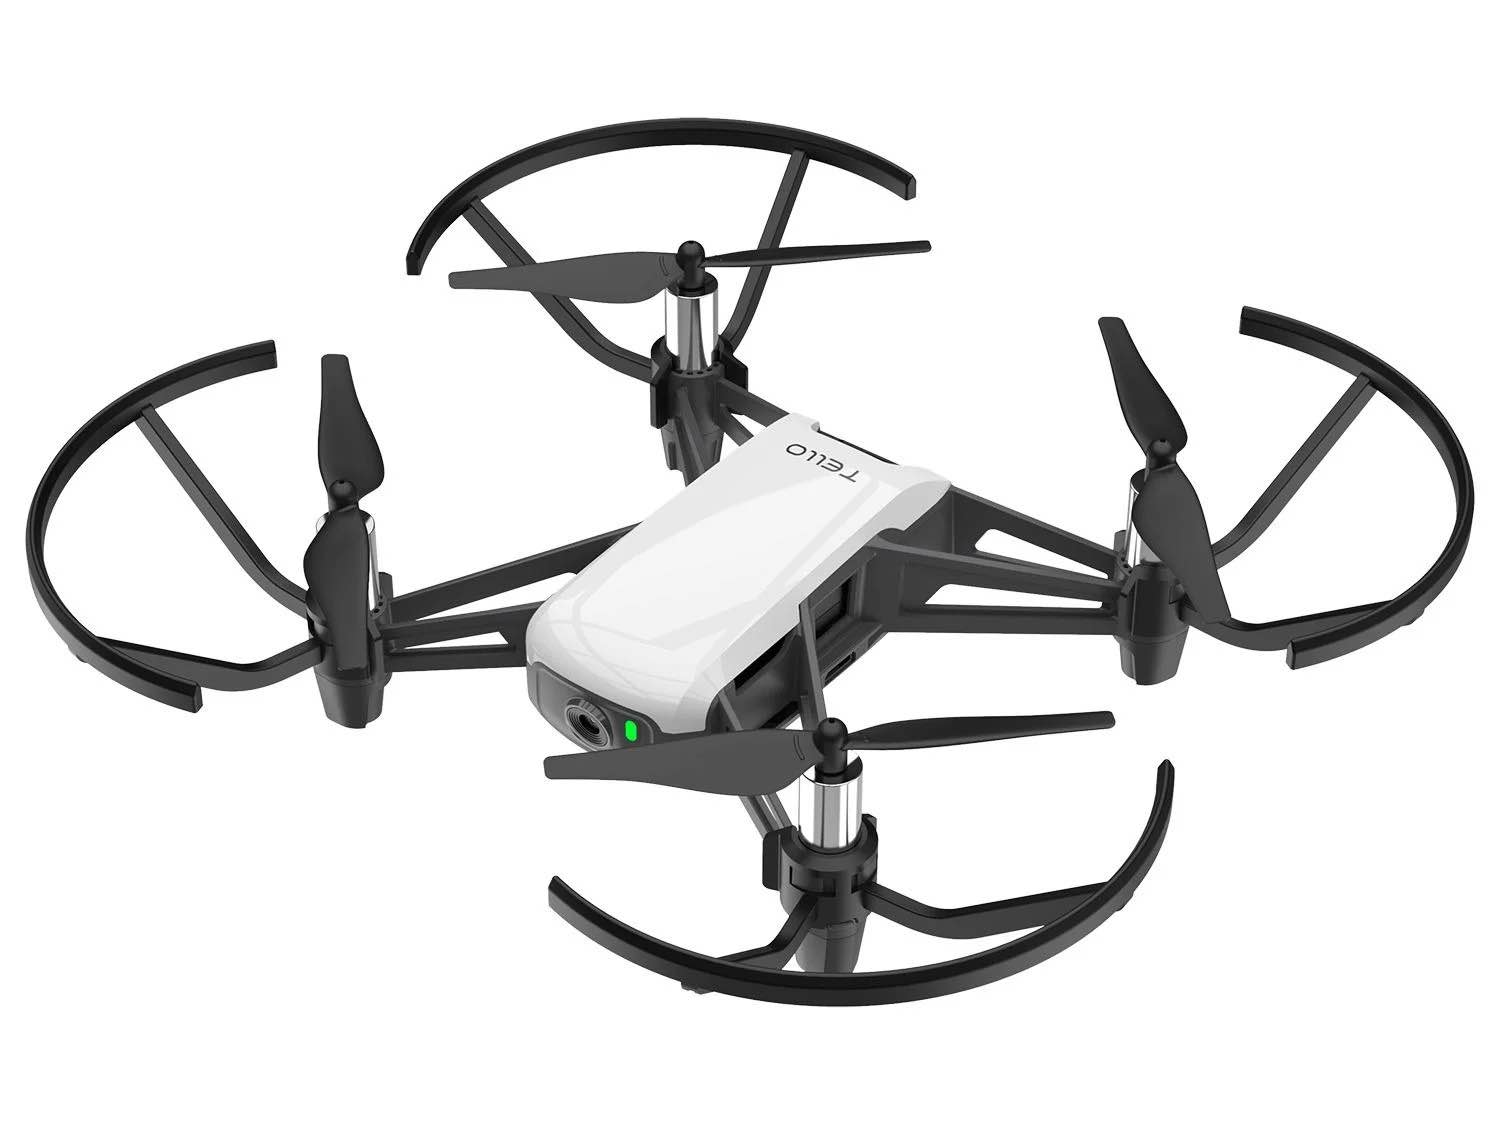
\includegraphics[scale=0.2]{figuras/dispositivo_utilizado.png}
  % \caption[Así aparece el rótulo en el índice]{Así aparece el rótulo en el texto.}
  \caption[DJI Tello. Dispositivo utilizado durante el proyecto]{Imagen del dispositivo utilizado durante el proyecto.}
  \label{fig-dron}
\end{figure}


El dispositivo cuenta con una cámara integrada con una resolución máxima de 1280x720 píxeles, la cual creemos que es suficiente para el desarrollo del trabajo.
\medskip

Un punto negativo del uso de drones como dispositivo de captura es el poco rendimiento de las baterías durante el vuelo. Concretamente, el dron utilizado permanece en vuelo unos 13 minutos como máximo.
\medskip

Además, durante el desarrollo inicial del proyecto se pudo observar una latencia reseñable al intentar comunicar el dispositivo con el ordenador a la hora de transmitir las imágenes y de poder enviar señales de control debido a la débil conexión WiFi entre ambos puntos de comunicación. El intentar solucionar este problema no solo consumió tiempo de ejecución del proyecto sino que también nos impide poder llevar a cabo pruebas de control más realistas y nos acotará el margen de ejecución de nuestras pruebas finales.
\medskip

\section{Marco teórico}

En esta sección haremos una breve introducción a los diferentes componentes teóricos que nos iremos encontrando a lo largo del trabajo. Empezaremos repasando los principales conceptos relacionados con el aprendizaje por refuerzo y en qué se diferencia de otros tipos de entrenamiento. 
\medskip

Después haremos una introducción a cada uno de los algoritmos que vamos a utilizar y comentaremos brevemente las diferencias y el por qué los elegimos.
Por último comentaremos los \textit{Transformers}\citep{transformers} y en especial los \textit{Vision Transformers}\citep{visiontransformers}, ya que serán utilizados durante uno de los experimentos que explicaremos en la sección \ref{experimentacion} .
\medskip

\subsection{Aprendizaje por refuerzo}
\label{aprendizaje-por-refuerzo}

\subsection{Algoritmo Policy Gradient}
\label{algoritmo-policy-gradient}

\subsection{Algoritmo Actor-Critic}
\label{algoritmo-actor-critic}

\subsection{Transformers y Vision Transformers}
\label{vision-transformers}

Sin entrar en muchos detalles en cuanto a cómo funcionan los \textit{Transformers} y los \textit{Vision Transformers}, haremos un breve repaso de las características unicas de estas redes, ya que uno de los experimentos nombrados en la sección \ref{resultados-vision-transformers} será el de un agente con una red de tipo \textit{Vision Transformer} \citep{visiontransformers}, que se encargará de realizar la transformación de la imagen de entrada.
\medskip

\begin{figure}[H]
  \centering
  \subfloat[Arquitectura \textit{Transformer} original]{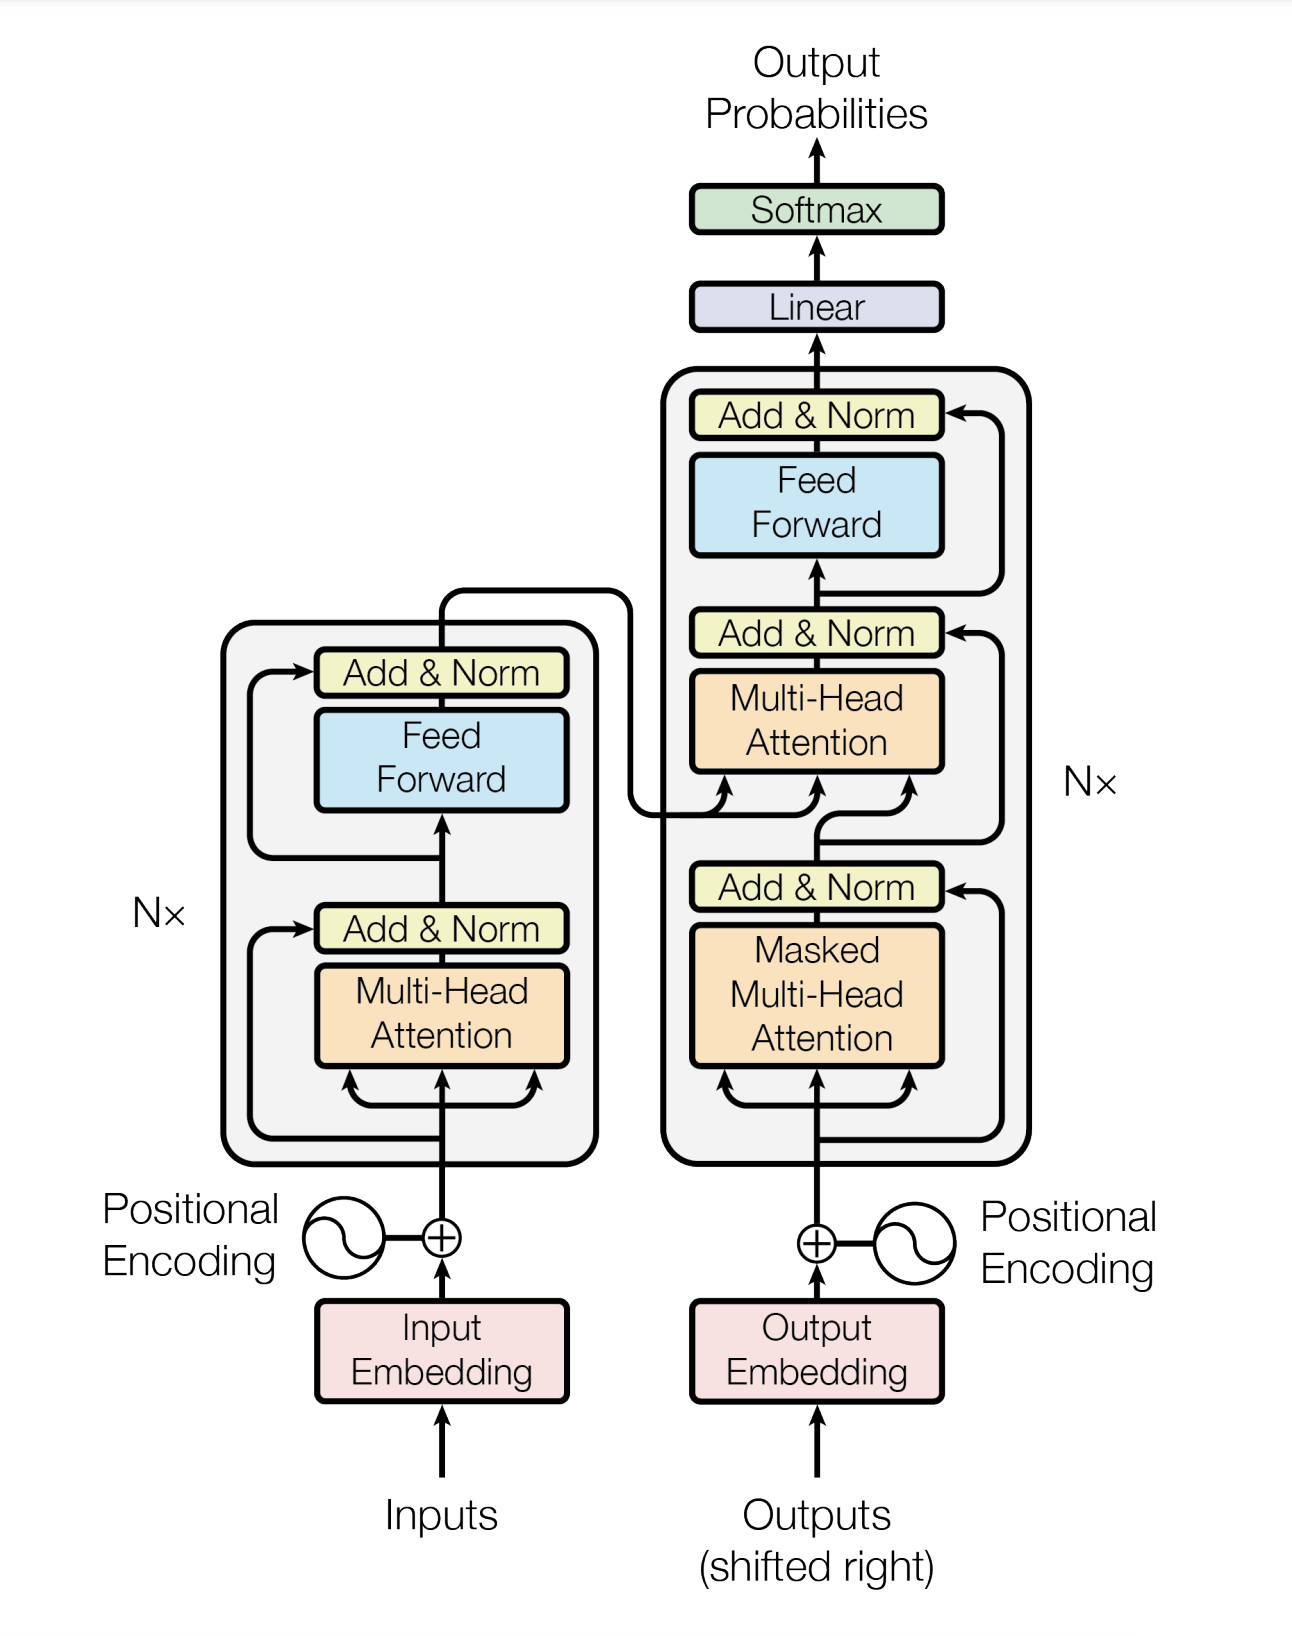
\includegraphics[scale = 0.2]{figuras/transformer_architecture.png}}
  \subfloat[Arquitectura propuesta para \textit{Vision Transformers}]{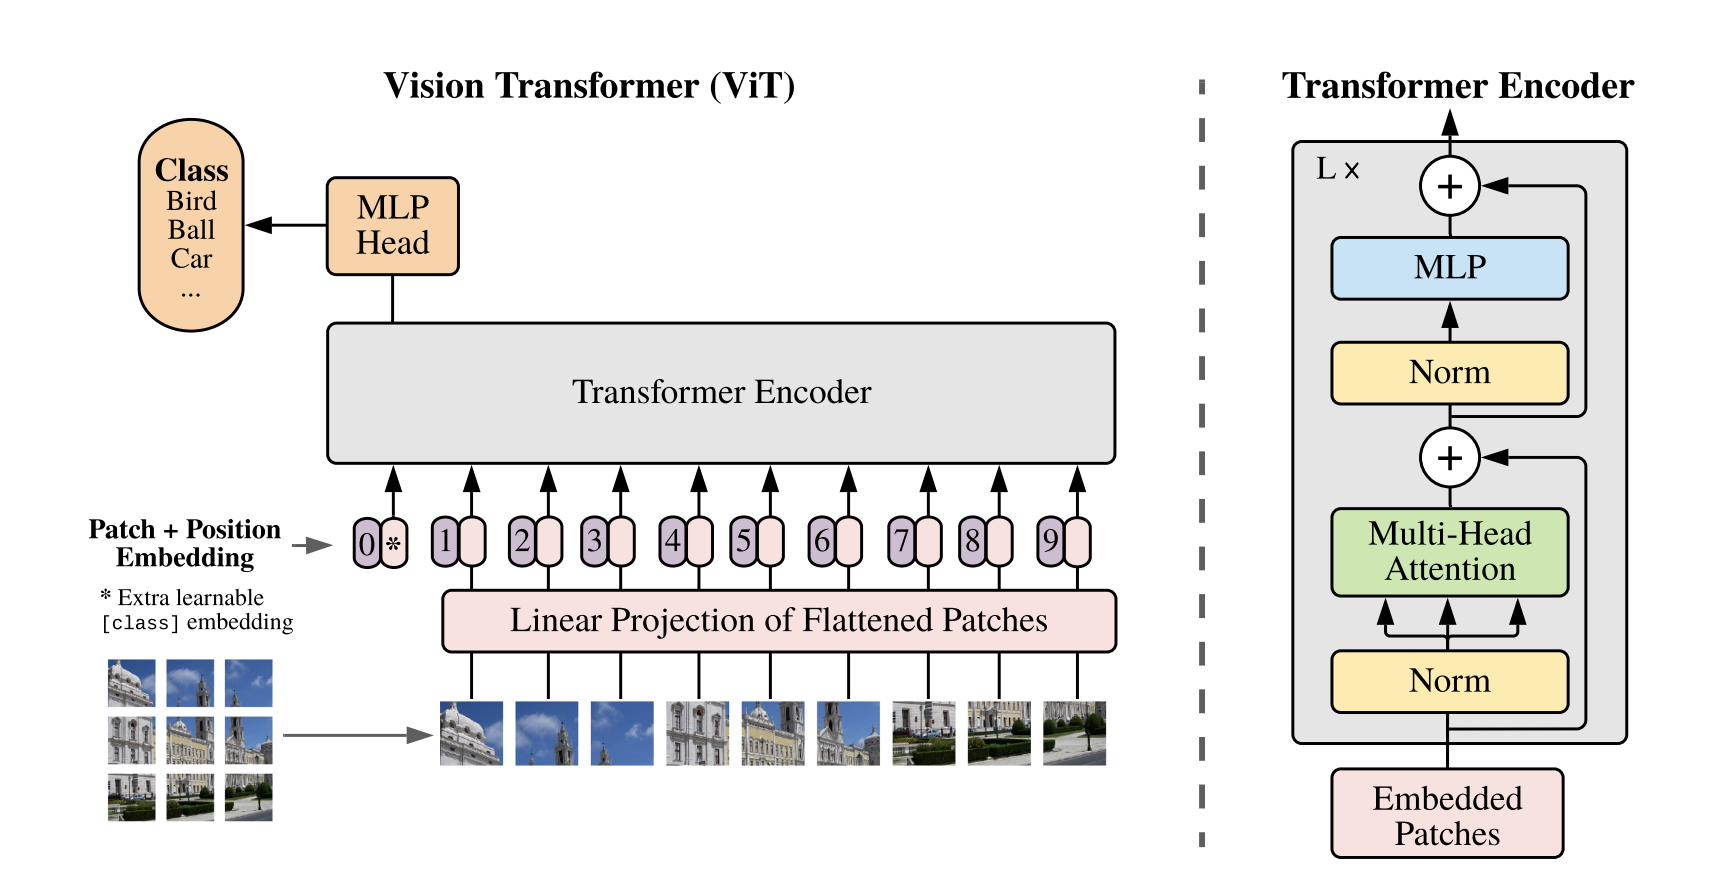
\includegraphics[scale = 0.3]{figuras/vision_transformers.png}} 
  % \caption[Así aparece el rótulo en el índice]{Así aparece el rótulo en el texto.}
  \caption[Comparativa arquitectura (a) Transformer y (b) Vision Transformer]{Comparativa arquitectura (a) Transformer y (b) Vision Transformer}
  \label{fig-vision-transformer}
\end{figure}

Las redes basadas en \textit{Attention}, en particular las redes \textit{Transformers}, desarrolladas inicialmente por Google, se han convertido en la elección por defecto en problemas de lenguaje natural o NLP, ya que gracias a su eficiencia computacional y su escalabilidad, es posible entrenar modelos de más de 100 billones de parámetros. La idea detrás de estas redes es solucionar los problemas que presentan las redes neuronales recurrentes o RNN, tales como las redes LSTM o GRU, las cuales no son capaces de captar dependencias a largo plazo, tal y como podemos encontrarnos en un texto de una novela.
\medskip

Aunque los \textit{Transformers} son ampliamente utilizados en procesamiento de lenguaje natural, las arquitecturas de redes convolucionales o \glossary{CNN} seguian siendo el tipo de red dominante en el campo de la visión por computador. Es por ello que, inspirados en la arquitectura original de Transformer y en el éxito que estas contaban (y aún cuentan), se buscó aplicar los mismos principios en la visión por computador. Esto es lo que dio lugar a los Vision Transformer, cuya idea principal es la de partir una imagen en segmentos o \textit{patches} y ser capaces de aplicar capas de Attention a cada uno de ellos. 
\medskip

A día de hoy nos encontramos muchas versiones disponibles y preentrenadas. Durante la ejecución de nuestro experimento utilizaremos un modelo disponible en la web \href{https://huggingface.co/docs/transformers/model_doc/vit#transformers.ViTModel}{HuggingFace}. En concreto utilizamos un modelo entrenado por Google, cuya entrada es una imagen de 224x224 píxeles, que será luego dividida en 16 parches de 14x14 píxeles y que fue entrenada en el conjunto de datos \textit{ImageNet21k} \citep{imagenet21k}. La salida de este modelo, es decir, la entrada a nuestro agente será un vector de tamaño 197x512, donde la primera dimensión representa el tamaño de la secuencia en la cual nuestra imagen ha sido partida tras el paso por el \textit{Vision Transformer}, y cada elemento de esa secuencia consta de un total de 512 características.
% OBJETIVOS

\cleardoublepage

\chapter{Objetivos}
\label{objetivos}

Describe aquí el objetivo general de tu Trabajo Fin de Máster y, a continuación, define los objetivos parciales:
\medskip
\begin{enumerate}[label=\destacado{\arabic*.}]
  \setlength\itemsep{1em}
  \item \textbf{Objetivo parcial 1.}

  \item \textbf{Objetivo parcial 2.}

  \item \textbf{Objetivo parcial 3.}
\end{enumerate}

% METODOLOGÍA

\cleardoublepage

\chapter{Metodología}
\label{metodologia}

\section{Obtención de los datos}
\label{obtencion-datos}

La toma de datos se hace mediante el análisis de archivos de vídeo tomados desde el propio dispositivo en un entorno controlado. Es importante destacar que la calidad de las imágenes no es alta, sobre todo en entornos en los cuales la iluminación no es favorable, por ejemplo en entornos con iluminación artificial. 
\medskip

El dispositivo nos proporciona una aplicación móvil para controlar la grabación y el almacenamiento de los videos que luego serán volcados en el ordenador para su posterior procesamiento, del cual hablaremos posteriormente.
\medskip

\begin{figure}[H]
    \centering
    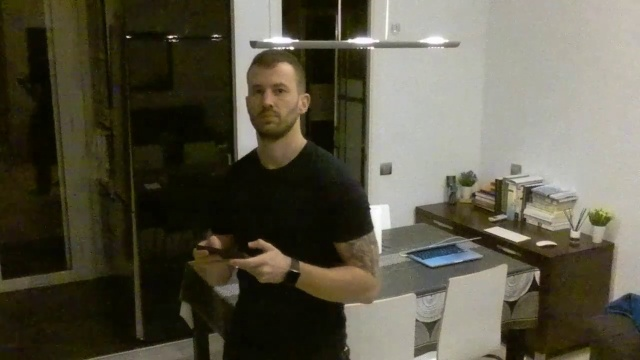
\includegraphics[scale=0.3]{figuras/dataset/image2.jpg}
    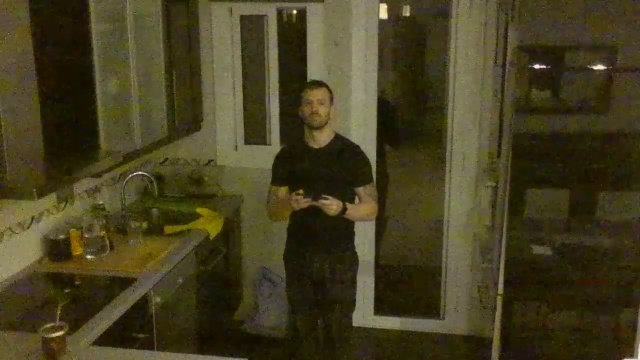
\includegraphics[scale=0.3]{figuras/dataset/image7.jpg}
    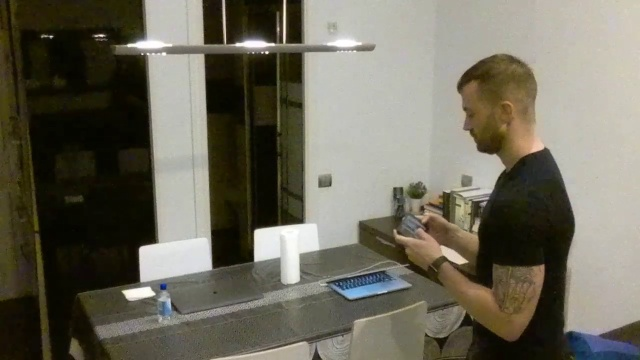
\includegraphics[scale=0.3]{figuras/dataset/image8.jpg}
    % \caption[Así aparece el rótulo en el índice]{Así aparece el rótulo en el texto.}
    \caption[Imágenes de ejemplo del conjunto final de datos]{Imágenes de ejemplo del conjunto final de datos.}
    \label{fig-dataset-imagenes-ejemplo}
\end{figure}
\medskip
Se ha decidido también utilizar sólo imágenes procedentes del dispositivo y no incluir imágenes de terceras fuentes que podrían haber ayudado a mejorar el tamaño final de nuestro conjunto de datos ya que la idea es acercarse lo máximo posible a un entorno final real.
\medskip

Debido a las leyes vigentes sobre vuelo de drones, los escenarios en los cuales fueron grabados los videos se redujeron drásticamente a un entorno cerrado, lo cual nos lleva a pensar que más adelante podríamos tener un problema de overfitting en nuestro modelo.
\medskip

En un escenario ideal contaríamos con diferentes entornos que nos permitiesen descartar la posibilidad de que el agente aprenda que la posición de determinados objetos es condicionante para tomar una decisión y que se centrara solo en las persona de la imagen.
\medskip

\section{Preprocesamiento de los datos}
\label{preprocesamiento-datos}
\begin{figure}[ht!]
    \centering
    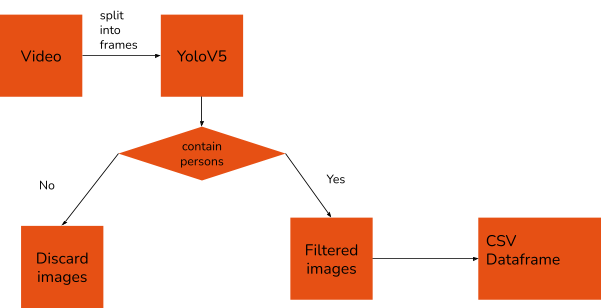
\includegraphics[scale=0.6]{figuras/data_preprocessing.png}
    % \caption[Así aparece el rótulo en el índice]{Así aparece el rótulo en el texto.}
    \caption[Pipeline del procesamiento del conjunto de datos]{Pipeline del procesamiento del conjunto de datos.}
    \label{fig-preprocesamiento-datos}
\end{figure}


Tras la recolección de videos y fotos desde el dispositivo, se realiza un primer proceso de filtrado. Este primer paso consiste en realizar un split de los archivos de video en frames individuales y realizar una operación de reducción del tamaño sobre los frames originales, pasando de 1280 píxeles de ancho y 720 píxeles de alto, a 640 píxeles de ancho y 360 píxeles de alto. Más adelante se tendrá que realizar una segunda reducción de las imágenes para adaptarlas al tamaño de entrada de la red convolucional previa al agente.
\medskip

Este primer paso de filtrado es posible gracias a los algoritmos de detección de objetos, mediante el uso de redes convolucionales neuronales, que nos proporcionan las coordenadas de las bounding box de aquellas clases de objetos que queremos encontrar en nuestro conjunto de datos.
\medskip

Durante el transcurso de nuestro proyecto utilizaremos \textit{YOLOv5}(\citep{youonlylookonce}), cuya implementación se encuentra disponible de forma gratuita como librería open source. Dicha implementación nos proporciona además múltiples configuraciones de la red. En nuestro caso, esto no fue muy relevante dado que solo lo utilizaríamos para una primera fase de preprocesamiento de las imágenes.
\medskip

Debido a que la red \textit{YOLOv5} fue entrenada sobre el conjunto de datos \textit{ImageNet} \citep{imagenet} para detectar 1000 clases de objetos diferentes, debemos modificarla para que sea capaz de detectar tan solo una persona en las imágenes que le pasamos, si es que la hay. La documentación de la librería nos ayuda a conseguir esto, de manera que tras una serie de pruebas tanto de diferentes arquitecturas de \textit{YOLO} como de configuración de los parámetros, en concreto: el intervalo de confianza y  el IoU threshold, la red nos devuelve la ubicación de la bounding box en donde se encuentra la persona si es que la hubiese.
\medskip

Sin embargo, para poder adaptar la salida de la red a nuestras necesidades, lo que hicimos fue calcular el punto central de la bounding box en coordenadas X e Y, para que nuestro agente intente acercarse a ese punto durante el entrenamiento en el menor número de pasos posible.
El resultado fue por un lado, un dataframe de Pandas que contenia la ruta de la imagen que \textit{YOLO} había filtrado y las coordenadas X e Y del punto central de la bounding box.
\medskip

Un punto a destacar es que las imágenes que no contenían personas fueron descartadas del conjunto de datos. Esta fue una decisión que se valoró al inicio con el fin de conseguir un agente y una definición más sencilla del problema. De no haber sido así, tendríamos que haber tenido en cuenta el hecho de que la imagen no presenta un punto objetivo y por lo tanto el dron debería permanecer quieto o girar hasta encontrar una persona.
\medskip

El número total de imágenes de nuestro conjunto de datos inicial tras este primer paso se reduce a tan solo 1690 imágenes. Sin embargo, y debido a que nuestro objetivo es modelar los movimientos de giro del dron tenemos que ser conscientes de cuántas imágenes contamos para que el dron nos detecte a la derecha, a la izquierda o en el centro de la imagen.
\medskip

En un primer análisis, nuestro conjunto de datos se encontraba completamente desbalanceado. Lo que hicimos para comprobar esto fue tomar las coordenadas centrales de la bounding box sobre el eje X que calculamos con \textit{YOLO} y comprobar en qué parte de la imagen se encontraba. Si esta coordenada se encontraba entre los píxeles 0 y 280, entonces el dron tendría que que girar a la izquierda, si se encontraba entre el 280 y el 360, entonces podríamos decir que el dron se mantendría prácticamente quieto, y si la coordenada se encontraba por encima de 360, el dron tendría que girar hacia la derecha.
\medskip

Los resultados de este análisis fueron los siguientes:

\begin{itemize}
    \item 340 imágenes se encontraban con la coordenada X en el lado izquierdo.
    \item 870 imágenes se encontraban con la coordenada X en el lado derecho.
    \item 480 imágenes se encontraban con la coordenada X en el centro de la imagen.
\end{itemize}

Debido a este desbalance, se tomó la decisión de igualar la cantidad de imágenes en cada lado, dejando un total de 340 imágenes por cada categoría, lo que hizo un total de 1020 imágenes finales para el entrenamiento y la validación de nuestro agente, lo que en contrapartida podría incrementar aún más el overfitting, pero nos aseguramos de que las decisiones que toma nuestro agente no se verán condicionadas por el número de acciones totales que debería tomar sobre un lado u otro. 
\medskip

Sin embargo, antes de tomar la decisión de descartar las imágenes se estudió la posibilidad también de realizar técnicas de data augmentation tal y como se recomienda en la literatura, utilizando técnicas de crop y volteo horizontal y vertical en cada una de las imágenes, pero la complejidad añadida de tener que recalcular el nuevo punto central hizo que descartemos esa posibilidad.
\medskip

Debido a que nuestro conjunto de datos no es muy grande, decidimos que el conjunto de entrenamiento sea el 90\%, del cual el 80\% se usará para la fase de entrenamiento de nuestro modelo y el otro 20\% se usará para la fase de test. El 10\% restante de nuestro conjunto, aproximadamente 100 imágenes, lo reservamos para la etapa de validación, de manera que probaremos los resultados de nuestro agente sobre un conjunto de imágenes que no haya visto previamente.



\section{Análisis de la solución e implementación}
\label{analisis-de-la-solucion-e-implementacion}

En la siguiente sección hablaremos de la implementación de cada uno de los elementos que componen nuestro problema, así como de las decisiones iniciales tomadas.
\subsection{Elección de los algoritmos utilizados por el agente}
\label{eleccion-de-algoritmos}

Para entrenar nuestro agente utilizaremos métodos que optimicen la \textit{policy} del agente, es decir, que optimicen la toma decisiones para maximizar la \textit{reward} del entorno.
\medskip

Comenzaremos utilizando el algoritmo \textit{REINFORCE Policy Gradient}, el cual se considera de los más sencillos dentro de la familia de \textit{Policy Gradient} y nos servirá como punto de partida para analizar los posibles problemas y limitaciones de nuestro entorno y nuestras definiciones. Con este algoritmo, el agente colecciona ejemplos del episodio utilizando para ello la \textit{policy} actual. La figura \ref{fig-algoritmo-reinforce} muestra dicho algoritmo:
\medskip
\begin{figure}[ht!]
	\centering
	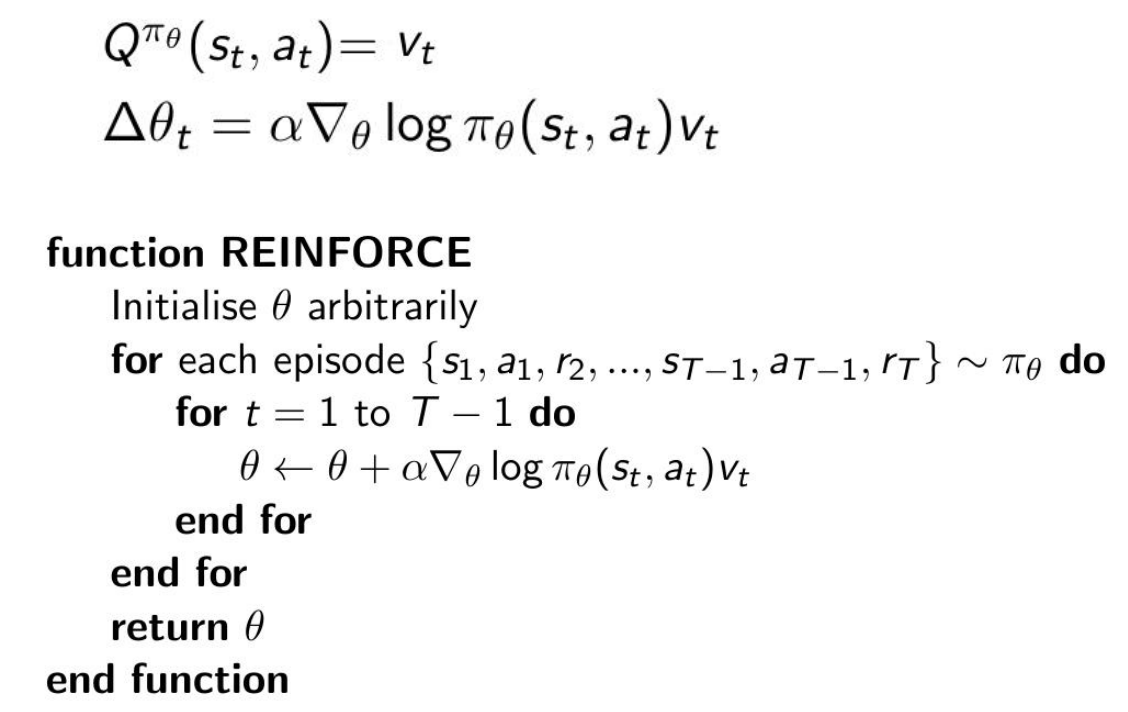
\includegraphics[scale=0.5]{figuras/reinforce_policy_gradient.png}
	\caption[Algoritmo REINFORCE Policy Gradient]{Algoritmo REINFORCE Policy Gradient. Obtenida de la \href{http://www.cs.toronto.edu/~tingwuwang/REINFORCE.pdf}{UToronto}}
	\label{fig-algoritmo-reinforce}
\end{figure}

Como siguiente paso, escogeremos nuevamente un algoritmo de la familia de \textit{policy gradient} para el entrenamiento del agente. En este caso, el algoritmo \textit{Actor-Critic} \citep{DBLP:journals/corr/abs-1801-01290}. La mayor diferencia entre este algoritmo y el anterior, es que en este caso contamos con 2 componentes separados: el \textit{Actor}, que será el responsable de devolver la distribución de probabilidades de cada una de las acciones del agente y el \textit{Critic}, que será el encargado d estimar el valor del estado en el que se encuentra dicho agente. El algoritmo utilizado puede verse en la figura \ref{fig-algoritmo-actor-critic}.
\medskip

\begin{figure}[ht!]
	\centering
	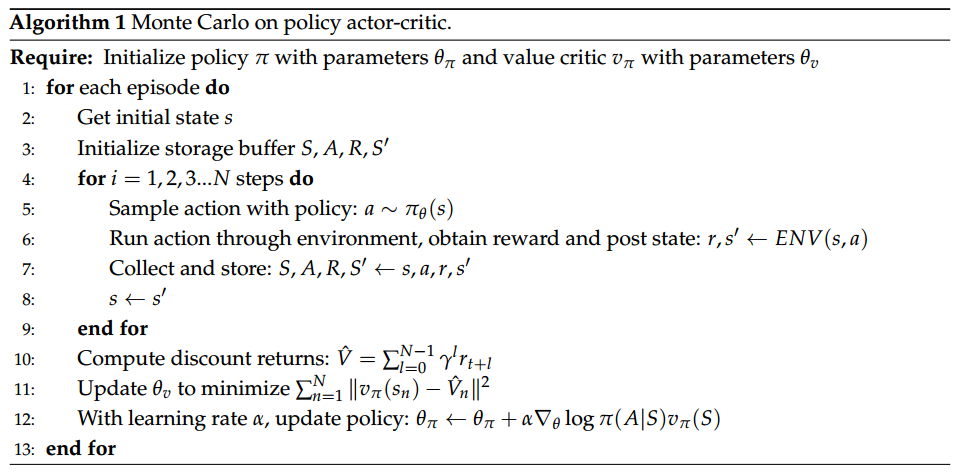
\includegraphics[scale=0.5]{figuras/algoritmo_actor_critic.png}
	\caption[Algoritmo Actor Critic]{Algoritmo Actor Critic. Obtenida de \href{https://preview.redd.it/6dfwcx17zwi21.png?width=971&format=png&auto=webp&s=e1f13781cf1b436425b8e7e802fc24b6a6951e8e}{Reddit}}
	\label{fig-algoritmo-actor-critic}
\end{figure}

\subsection{Definición del estado}
\label{definicion-del-estado}

El estado es la representación del problema que el agente debe resolver. En este caso, el estado será una imagen de la cámara del dron, a la que se le aplicó previamente un procesamiento, tal y como comentamos en la sección \ref{preprocesamiento-datos}, junto con el punto en el que se encuentra el agente, expresado en un número entre 0 y 1, representando el 0 estar en el borde izquierdo de la imagen y 1 estar en el borde derecho de esta.
\medskip

Es decir, el agente recibirá un vector como entrada, de tamaño 4097. Los primeros 4096 elementos representan la imagen, la cual ha sido procesada por una \acrshort{cnn} preentrenada, que en nuestro caso ha sido VGG16 \citep{vgg16}, la cual recibe como entrada un vector de tamaño 224x224x3, es decir, una imagen en formato RGB de 224x224 píxeles. Si bien la elección de nuestra \acrshort{cnn} no fue basándonos en ningún criterio en particular, la idea era disminuir el tamaño de la entrada de nuestro agente. 
\medskip

También se tuvieron en cuenta diferentes soluciones para la definición del estado. Entre ellas, la posibilidad de que el estado se formase de varias imágenes al mismo tiempo, debido el componente temporal con el que cuenta nuestro problema. Este estado condicionaría también la arquitectura de la red de nuestro agente, dado que en este caso necesitaríamos tratar con redes recurrentes o en su defecto con redes de tipo Transformers \citep{transformers}, tal y como se explica en el trabajo realizado por \citet{luo2019end} y podemos ver en la figura \ref{fig-arquitectura-red-luo}, donde podemos ver que después del \textit{encoder}, tal y como se cita en el trabajo, se utiliza una red \acrshort{LSTM}.
\medskip

\begin{figure}[H]
    \centering
    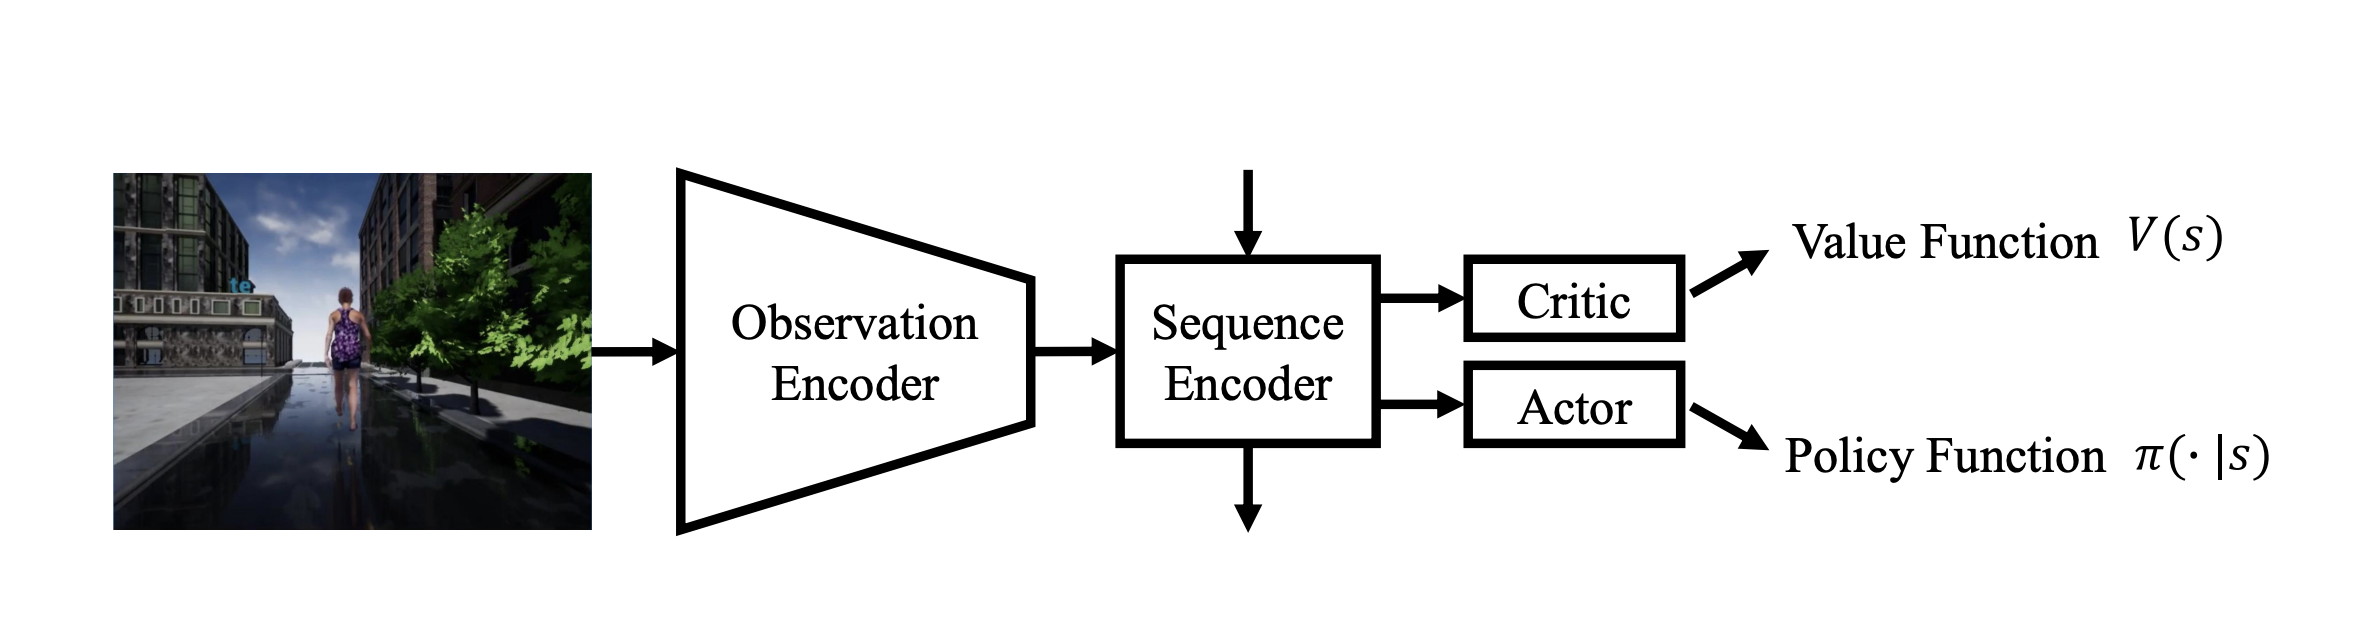
\includegraphics[scale=0.3]{figuras/luo_network_architecture.png}
    % \caption[Así aparece el rótulo en el índice]{Así aparece el rótulo en el texto.}
    \caption[Arquitectura de red propuesta por \citet{luo2019end}.]{Arquitectura de red propuesta por \citet{luo2019end}.}
    \label{fig-arquitectura-red-luo}
\end{figure}

Para aumentar la velocidad de nuestro entrenamiento, la imagen será preprocesada por la red convolucional al inicio de cada episodio y se mantendrá constante, dado que lo que iremos cambiando con cada acción durante el entrenamiento es el punto en el que se encuentra el agente.
\medskip

Por último, el estado contiene en su último elemento, el punto en el que se encuentra el agente en un momento dado, de manera que este debería ser capaz de tomar decisiones basándose no solo en la representación de la imagen sino también del valor que este valor tenga en ese instante.

\subsection{Definición de la recompensa}
\label{definicion-de-recompensa}

El desarrollo de la recompensa fue uno de los puntos críticos en cuanto a la implementación y la definición de nuestro problema. Por un lado, tenemos que intentar que nuestro agente sea capaz de ir aprendiendo los pasos intermedios que lleven a la obtención de la recompensa óptima, en el menor número de pasos posibles y por otro, definir cúanta recompensa en términos absolutos el agente recibirá cuando acaba correctamente el episodio, en contraposición a cuando llega al número máximo de intentos sin haber obtenido la recompensa máxima.
\medskip

La idea inicial fue crear una zona de recompensa proporcional a la distancia del punto en el que se encontraba el agente y el punto obtenido durante el preprocesamiento de los datos. Esto lo hicimos diviendo la imagen en secciones longitudinales de tamaño fijo. Dado que nuestra imagen era de 640 píxeles de ancho, lo que hicimos fue dividirla en 32 secciones de 20 píxeles cada una. La recompensa final obtenida sería inversamente proporcional a la distancia, medida en número de secciones, en que el agente se encontraba con respecto al punto objetivo. De manera que si el agente se encontraba a 5 secciones de nuestro punto final, obtendría menos recompensa que si se encontrara a 2 secciones, tal y como se puede observar en el algoritmo \ref{algrecompensainicial}:
\medskip
\vspace{3ex}
\begin{algorithm}[H]
\label{algrecompensainicial}
\SetAlgoLined
\medskip
\begin{enumerate}
	\item Dividimos la imagen en secciones longitudinales de tamaño fijo $Secciones_{total}$.
	\item Establecemos una recompensa máxima del entorno $Recompensa_{max}$.
	\item Calculamos la sección en la que se encuentra nuestro agente:
	$Seccion_{agente} = round(Pagente_{pixels} / Ancho_{imagen})$.
	\item Calculamos la sección en la que se encuentra nuestro punto final:
	$Seccion_{objetivo} = round(Pobjetivo_{pixels} / Ancho_{imagen})$.
	\item Si $Seccion_{agente} = Seccion_{objetivo}$ devolvemos $Recompensa_{max}$.
	
	Sino devolvemos $1 - (Seccion_{agente}-Seccion_{objetivo}/Secciones_{total}) $
\end{enumerate}
	\caption{Algoritmo de recompensa inicial}
\end{algorithm}
	
\vspace{3ex}

Lo que conseguimos con esta recompensa fue obtener un \textit{heatmap} alrededor del punto objetivo, de manera que el agente podría interpretar si se estaba acercando o alejando. 
\medskip

La recompensa máxima fue establecida a 1, de manera que los saltos entre las recompensas parciales y la recompensa final fuese siempre proporcional a la distancia. Más adelante también comprobaremos cómo este valor puede afectar al desarrollo de una solución por parte de nuestro agente.
\medskip

\begin{figure}[ht!]
	\centering
	\parbox{5in}{
		\centering
		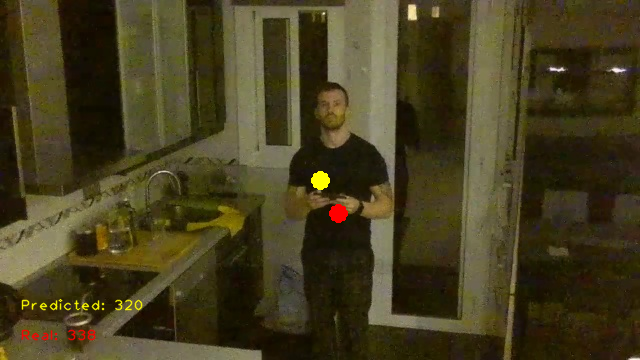
\includegraphics[scale=0.35]{figuras/recompensa/recompensa_maxima.png}
	}
	\qquad
	\begin{minipage}{5in}
		\centering
		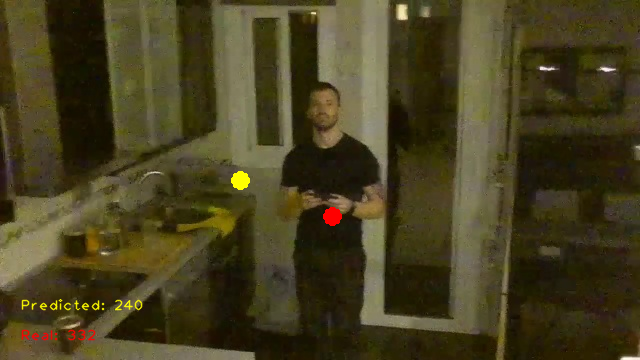
\includegraphics[scale=0.35]{figuras/recompensa/recompensa_no_maxima.png}
	\end{minipage}
	\caption[Comparación de recompensa sobre la misma imagen dados dos puntos de vista distinto.]{La misma imagen, con 2 puntos definidos por el agente a diferente distancia del punto objetivo. La imagen superior obtendría la puntuación máxima mientras que la imagen inferior no.}%
	\label{fig-recompensa-imagenes}
\end{figure}


En la figura \ref{fig-recompensa-imagenes} podemos observar cómo funciona nuestro sistema de recompensa inicial. En la imagen situada en la parte superior, el punto amarillo, que representa el punto en el que se encuentra el agente, está dentro de la misma sección que el punto objetivo, y por lo tanto la recompensa será máxima. Mientras que en el caso de la imagen inferior, el punto donde se encuentra el agente está a una distancia mayor a una sección (definida por defecto en 20 píxeles), y por lo tanto la recompensa será proporcional al número de secciones que se encuentra hasta llegar al punto objetivo.

\subsection{Definición del entorno}
\label{definicion-del-entorno}

Para desarrollar el entorno, lo que se hizo fue implementarlo siguiendo como ejemplo los entornos propuestos por OpenAI Gym \citep{openaigym}. Esto nos facilitó tener una primera estructura y una primera definición de los métodos que deberíamos implementar.
\medskip

Al inicio de cada episodio, nuestro entorno se encargará de devolver una imagen del conjunto de datos (entrenamiento, test o validación), así como las coordenadas del punto en el que se encuentra la persona, expresados en píxeles, que es lo que compone nuestro estado tal y como describimos en la sección \ref{definicion-del-estado}. Estos valores se guardan durante toda la ejecución del episodio y se renuevan una vez que se empieza uno nuevo.
\medskip


La ejecución de cada acción sobre el entorno nos devolverá un nuevo estado, la recompensa asociada con ese estado y un valor que nos indicará si el estado es final o no, es decir, si el episodio finaliza en ese estado. 
\medskip

El algoritmo \ref{environment-step-action} detalla el pseudocódigo utilizado tras recibir una acción por parte del agente. Podemos observar que este algoritmo mueve el punto del agente basándose en la acción que este toma, siempre en una cantidad fija de píxeles, que corresponde con el tamaño de cada una de las secciones en las que fue dividida la imagen tal y como se explica en el apartado \ref{definicion-de-recompensa}. Esto se hizo de tal forma que el agente se moviese siempre a una sección diferente y por lo tanto la recompensa obtenida también sea diferente.
\medskip

\vspace{3ex}
\begin{algorithm}[H]
	\label{environment-step-action}
	\SetAlgoLined
	\medskip
	$width \gets 640$

	$distance \gets 20$

	\If{accion == 'LEFT'}{
		$point \gets point - distance$
	}
	\If{action == 'RIGHT'}{	
		$point \gets point + distance$
	}
	$point \gets torch.clamp(point, 1, width-1)$

	$reward \gets calculateReward(point)$

	$done = EnvironmentMaxReward == reward$

	\Return{reward, point, done}
	\caption{Ejecutar acción en el entorno}
\end{algorithm}
\vspace{3ex}

Podemos observar también que la acción de permanecer quieto no tiene ninguna consecuencia en el estado del agente y la utilizaremos como posible acción para finalizar el episodio por parte del agente.
\medskip

Durante las fases de entrenamiento, testeo y validación de nuestro agente, cada una de las acciones sobre el entorno involucra el cálculo de la nueva posición del punto en el que se encuentra el agente. Una vez el agente fuese desplegado para controlar el dron, cada ejecución de la acción involucraría la ejecución de esa acción en el dron, ya sea girar a la derecha, a la izquierda, o permanecer quieto y obtener una nueva imagen. En este caso, el punto de vista del dron siempre sería el centro de la imagen.
\medskip

\subsection{Definición del agente}
\label{definicion-del-agente}

El agente es el componente que se encarga de tomar decisiones. En este caso, el agente será el encargado de tomar la decisión de girar la cámara del dron a la izquierda, a la derecha o de permanecer quieto, dado un estado del entorno, el cual está definido como se detalla en la sección \ref{definicion-del-estado}.
\medskip

El objetivo de nuestro agente será encontrar aquellas acciones que maximicen las recompensas obtenidas. Este objetivo será alcanzado dependiendo del algoritmo que utilicemos para ello, pero independientemente de esto, las recompensas obtenidas y el conjunto de acciones será el mismo.
\medskip

En cuanto a la implementación, el agente será una red neuronal cuya arquitectura iremos variando según los diferentes experimentos, que extenderá de la clase nn.Module de PyTorch y a la cual le añadiremos métodos propios para facilitar la lectura del código.


\subsection{Entrenamiento}
\label{entrenamiento}

En cuanto al proceso de entrenamiento, destacamos el hecho de que cada episodio está compuesto por una sola imagen. Es decir, cuando el agente llegue a la recompensa máxima establecida en cada imagen o cuando se llegue al número máximo de acciones que definimos durante el bucle de ejecución, el episodio acabaría. 
\medskip

La inclusión de un número máximo de pasos por imagen fue una decisión tomada para que nuestro agente no entrase en un bucle infinito si decidiese por ejemplo, girar siempre hacia la derecha, llegando al extremo de la imagen donde no se encuentra la persona. Esta decisión también nos lleva a experimentar con un parámetro extra en nuestro entrenamiento, ya que un número muy elevado de acciones puede llevarnos a que el agente no aprenda correctamente y por lo tanto la exploración sobre el entorno no tenga ningún efecto, y por otro lado, un número muy pequeño podría llevarnos a que el agente no tuviese el tiempo suficiente para aprender la policy adecuada dado el estado. Por lo general, este valor oscilaba entre 50 y 100 acciones por imagen, aunque también se realizaron pruebas con valores menores y mayores a estos.
\medskip

Debido al problema de la falta de imágenes en diferentes entornos, tal y como comentamos en la sección \ref{preprocesamiento-datos}. Se tomó la decisión de que el punto inicial se inicialice de manera aleatoria, entre un valor de 0 y 1, que luego será multiplicado por el ancho de la imagen para darnos las coordenadas reales y calcular la recompensa en ese punto. La idea detrás de esta decisión es dotar al entrenamiento de un componente aleatorio y por lo tanto evitar que nuestro agente pueda realizar overfitting sobre el conjunto de datos, dado que para una misma imagen , durante el entrenamiento, el punto de partida sea diferente.
\medskip

Durante el proceso de entrenamiento se realizaron multitud de pruebas, no solo en lo que respecta a los parámetros de nuestro modelo, sino también a los criterios de parada de cada episodio, el número máximo de acciones a tomar o la recompensa obtenida al seleccionar la acción de permanecer quieto. De estas diferentes decisiones hablaremos en cada uno de los experimentos.
\medskip

\subsection{Evaluación}
\label{evaluacion}

Para evaluar la calidad de los resultados del agente, comprobaremos sobre cada imágen del conjunto de validación, cuándo el agente decide quedarse quieto y la recompensa que obtiene al hacerlo. Esto se asemeja al comportamiento real que tendría al ser desplegado en el dron.
\medskip

La evaluación comienza con las coordenadas del punto del agente en las coordenadas centrales de la imagen, de manera que simula el punto central de la cámara del dron. Lo que se hace a continuación es ejecutar el agente sobre ese estado y aplicar las acciones de este hasta encontrarnos con la acción de permanecer quieto, lo cual sería el indicador de que el agente se encuentra en la posición en la que se encuentra la persona. En ese momento, dado que contamos con las coordenadas reales obtenidas durante el procesamiento, calculamos la recompensa.
\medskip

Esta operación se realiza tanto para el conjunto de test durante el entrenamiento, como para el conjunto de validación después del entrenamiento. En ambos casos, nuestro modelo funciona en modo evaluación y por lo tanto no se propagan cambios a los pesos de este.
\medskip

Además de la recompensa total, nos interesa en este caso obtener un agente que decida moverse de manera uniforme hacia una dirección en el menor número de acciones posible. Pensemos que cada acción que tome el agente será una acción que el dispositivo tendrá que realizar y por lo tanto es tiempo de ejecución que se pierde. Es decir, un agente que consigue la recompensa máxima en 5 acciones será más valioso que uno que la consiga en 10.
\medskip

Aunque el hecho de conseguir la recompensa máxima del entorno en nuestro caso no es indicativo de la calidad de nuestro agente, por ejemplo podemos pensar que nuestro agente se acerca al punto en el que se encuentra la persona, sin llegar a estar exactamente en donde debería, pero sin embargo lo hace de manera consistente, en un número de acciones reducido por frame, lo que al final nos permite ser más rápidos en la ejecución final y por lo tanto, a efectos prácticos, nos puede incluso llegar a ser más valioso.
\medskip

\begin{figure}[ht!]
	\centering
	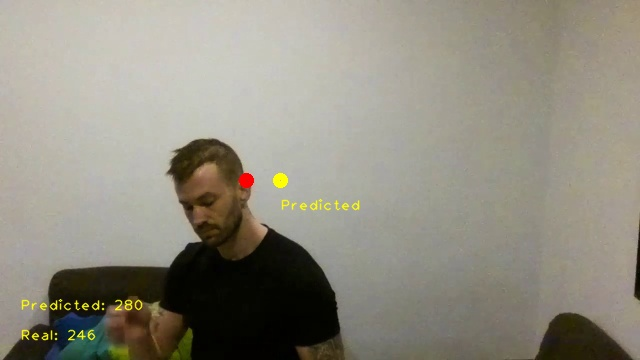
\includegraphics[scale=0.3]{figuras/recompensa/comparacion_2_acciones_tomadas.jpg}
	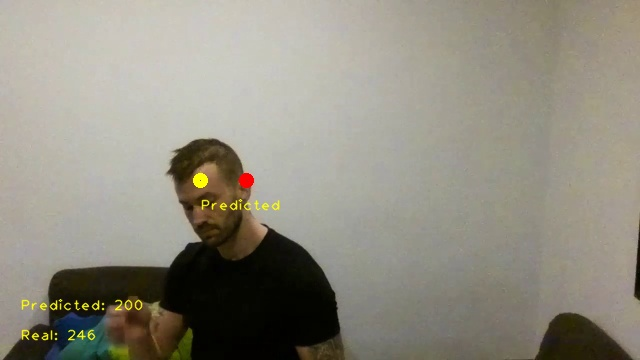
\includegraphics[scale=0.3]{figuras/recompensa/comparacion_6_acciones_tomadas.jpg}
	\caption[Imagen ejecutada en dos experimentos distintos, a la misma distancia del punto objetivo, con diferente número de acciones.]{Imagen ejecutada en dos experimentos distintos, cuyo punto predicho se encuentra a la misma distancia del punto objetivo, con diferente número de acciones.}%
	\label{fig-comparacion-numero de acciones}
\end{figure}

Un ejemplo de este comportamiento lo vemos en la figura \ref{fig-comparacion-numero de acciones}, en el que se puede ver que sobre la misma imagen, ejecutada en 2 experimentos diferentes, tenemos 2 puntos de vista por parte del agente a prácticamente la misma distancia. La imagen de la izquierda requirió de solamente 2 acciones, mientras que la imagen de la derecha de 6 acciones. Por lo tanto, para esta imagen nos interesaría el agente que produjo la imagen de la izquierda.
\medskip

Debido a la alta latencia que se producia al conectar el dron con nuestro ordenador, la ejecución en el dispositivo real no fue posible. Lo que se hizo en su lugar fue analizar frame por frame una serie de videos grabados desde el dispositivo, ejecutabdi una acción en cada uno de ellos para que simulara la acción a tiempo real que tomaría el agente.
Todos estos factores están sujetos a una evaluación subjetiva que iremos comentando más adelante en los diferentes experimentos que realicemos.
% RESULTADOS Y DISCUSION 

\cleardoublepage

\chapter{Resultados y Discusión}
\label{resultados-y-discusion}

\section{Introducción}
\label{resultados-introduccion}

A continuación haremos un repaso de los resultados obtenidos en el subconjunto de experimentos más representativo, realizados con los diferentes algoritmos propuestos.
\medskip

Detallaremos también las conclusiones parciales que obtenemos en cada experimento, así como posibles soluciones a los problemas que se nos plantean en cada uno.
\medskip

Cabe mencionar que debido al coste computacional de ejecutar cada experimento sobre el conjunto de datos total, cada experimento se compone de subexperimentos previos, en los cuales intentábamos probar nuestras soluciones con un conjunto de datos menor al original, alrededor de unas 20 imágenes. 
\medskip

La idea detrás de esta subexperimentación era conseguir un modelo de agente que sea capaz de realizar overfitting sobre el conjunto de datos de manera relativamente rápida y que obtuviese una convergencia tanto en la recompensa obtenida tanto en las imágenes del conjunto de entrenamiento como en el conjunto de test como en el número de pasos que realizaba sobre cada una de las imágenes. Esto nos permitió también acortar el tiempo entre las diferentes pruebas, lo que provocó que pudiesemos experimentar con diferentes definiciones tanto de nuestra recompensa como de nuestro entorno, así como hacer fine tunning de nuestros hiperparámetros.
\medskip

El total de los experimentos está disponible en el repositorio de \href{https://github.com/lucaswerner90/msc-degree-ai}{GitHub} para un análisis más extenso y se adjunta el título de cada uno de ellos en el Apéndize \ref{apendize-a}. 
\medskip

La herramienta utilizada para monitorear el progreso de las diferentes métricas durante los diferentes entrenamientos es \href{https://www.tensorflow.org/tensorboard?hl=es-419}{Tensorboard}, ya que además de su facil integración con \href{https://pytorch.org/}{PyTorch} nos permitía comparar dichas métricas entre los diferentes experimentos.


\section{Policy Gradient}
\label{resultados-policy-gradient}

\section{Actor Critic}
\label{resultados-actor-critic}

\section{Vision Transformers}
\label{resultados-vision-transformers}

% CONCLUSIONES

\chapter{Conclusiones}
\label{conclusiones}

\begin{enumerate}[label=\destacado{\arabic*.}]
  \setlength\itemsep{1em}
  \item Conclusión 1.

  \item Conclusión 2.

  \item Conclusión 3.
\end{enumerate}

% LIMITACIONES Y PERSPECTIVAS DE FUTURO

\cleardoublepage

\chapter{Limitaciones y\\ Perspectivas de Futuro}
\label{limitaciones-y-futuro}

En este capítulo hablaremos de las limitaciones con las cuales nos encontramos a la hora de desarrollar nuestro trabajo y haremos un análisis de los principales puntos que podrían mejorarse en futuras exploraciones.
\medskip

Comenzaremos hablando de los datos. Por regla general podemos asociar que un buen conjunto de datos marca la diferencia en el aprendizaje de una red neuronal profunda, no solo por su cantidad sino también por la variedad y la veracidad de estos comparados con un entorno real. En cuanto al último punto creo que se tomó la decisión correcta, ya que utilizamos imágenes capturadas por el propio dispositivo con el cual esperábamos usar nuestro agente y por lo tanto la calidad de las imágenes sería la misma. Sin embargo, es posible que nos hayamos quedado cortos en cuanto a la variedad de los escenarios, lo cual hizo que ya desde un principio tuviesemos que pensar que el \textit{overfitting} podría llegar a ser un problema. Esto podría ser facilmente solucionable si procesamos imágenes de diferentes entornos, de manera que nos aseguramos que el agente aprende realmente sobre el problema y no el entorno.
\medskip

Otro punto que supuso una limitación importante fue la limitada capacidad computacional con la que entrenamos nuestros agentes. En un principio se hicieron pruebas utilizando Google Colab, pero la limitación en cuanto a tiempo y el \textit{workflow} al cual nos obligaba a recurrir, hizo que lo descartasemos. También valoramos el uso de una máquina con procesadores gráficos compatibles con la librería \textit{PyTorch}, pero su costo operativo también hizo que no fuese una opción viable.
\medskip

También tenemos que hablar de nuestra falta de experiencia en el desarrollo de estos algoritmos y en general en la rama del aprendizaje por refuerzo, lo cual hizo que sumadas a las dificultades técnicas tuviesemos también que repasar los conceptos aprendidos en multitud de ocasiones.
\medskip

Pensando en trabajos futuros en esta línea de trabajo, dejamos abierta la posibilidad de usar algoritmos que nos ofrezcan una mejor convergencia en los resultados. Un ejemplo de esto podría ser la implementación de los algoritmos \textit{A2C} y \textit{A3C} \citep{DBLP:journals/corr/MnihBMGLHSK16}, que nos ofrecen la posibilidad de realizar múltiples entrenamientos al mismo tiempo o incluso podríamos pensar en la combinación de diferentes técnicas de inteligencia artificial como podrían ser el aprendizaje no supervisado o incluso la utilización de algoritmos genéticos para ayudarnos a encontrar una estructura de red óptima de nuestro problema \citep{cai2018efficient}. 

\cleardoublepage
\phantomsection

\printglossary[type=\acronymtype]
\printglossary

\appendix
% APÉNDIZES

% Escribe cada apéndize como si fuera un capítulo más.

\chapter{Apéndize A}
\label{apendize-a}

El siguiente apéndize muestra el conjunto de experimentos totales realizados durante la ejecución del proyecto. Cada uno de los experimentos se puede encontrar dentro de la carpeta runs/ del código del proyecto en el repositorio de \href{https://github.com/lucaswerner90/msc-degree-ai}{GitHub}.
\medskip

\begin{enumerate}
	\item Actor-Critic-ac-continuous-action
	\item Actor-Critic-ac-discourage
	\item Actor-Critic-ac-discourage-reward-1
	\item Actor-Critic-ac-discourage-reward-2
	\item Actor-Critic-ac-discourage-stop-action
	\item Actor-Critic-ac-no-rewards-till-complete
	\item Actor-Critic-ac-no-rewards-till-complete-divided
	\item Actor-Critic-ac-no-rewards-till-complete-full-training
	\item Actor-Critic-ac-reduce-reward-by-four
	\item Actor-Critic-ac-reward-2-divide-rewards-lr-e6
	\item Actor-Critic-ac-reward-2-min-3-disc-none-only-1000-steps
	\item Actor-Critic-ac-reward-2-min-actions
	\item Actor-Critic-ac-reward-2-min-actions-3-discount-none-only
	\item Actor-Critic-ac-reward-2-normalized-dataframe
	\item Actor-Critic-ac-reward-2-normalized-dataframe-lr-e7
	\item Actor-Critic-ac-reward-2-rew-by-two-stop-with-none
	\item Actor-Critic-ac-reward-2-rew-by-two-stop-with-none-only
	\item Actor-Critic-ac-vit-encoder
	\item Actor-Critic-no-sigmoid-state-value-adam-l2-reg-30steps-per-image-no-limit
	\item Actor-Critic-no-sigmoid-state-value-adam-l2-reg-30steps-per-image-stop-action
	\item Actor-Critic-softmax-state-value-adam-l2-reg-30steps-per-image-stop-action-is
	\item Actor-Critic-softmax-state-value-rmsprop-30steps-per-image-stop-action-is-non
	\item Actor-Critic-v1
	\item Actor-Critic-v2
	\item Policy gradient normalized image rewards
	\item Policy gradient normalized image rewards v2
	\item Policy gradient recompensa 10
	\item softmax-state-value
\end{enumerate}


\begin{singlespace}
\begin{footnotesize}
\begin{twocolumn}
\bibdata{bibliografia}
\bibliography{bibliografia}
\addcontentsline{toc}{chapter}{Bibliografía}
\end{twocolumn}
\end{footnotesize}
\end{singlespace}

\end{document}
